\section{Case and Results}
\label{method}
In this section the setup of the CFD analysis will be discussed. This includes the generation of the obstacles for the CFD analysis, a discussion on the Reynolds number associated with this geometry and the fluid properties used during the simulation. Our goal is to see if there is any updraft around 1 meter height, because if there is, that would mean skirts will be blown away in the wind. 
\subsection{Obstacle creation}
\label{obstacles}
To be as true to reality as possible (within the scope of the research practicum), not only the Flatiron building was simulated, but also 4 of the surrounding buildings, creating the ``alley'' of wind talked about in the introduction and \cite{dresses}. The dimensions of the Flatiron building itself were found in Bradford and Condit's book ``Rise of the New York Skyscraper 1865-1913'' \cite{skyscraper}, while the other dimensions were roughly estimated from Google Maps (see appendix \ref{appendixdimensions} for a clarification of the method and a complete list of dimensions used). \\
\indent %
The program used makes use of an ``obstacle generator'', in which you specify the start and end of the obstacle in the x, y and z direction, creating rectengular cuboids as obstacles. By combining multiple obstacles together, more complex shapes can be created. By discretizing a right angled triangle, the Flatiron building has been built up of 58 blocks of 1 metre wide, all varying in length to build up the triangle. The height of the building is uniform. The other buildings were 58 metres long and 25 metres wide. \\
\subsection{Mesh}
\label{sec:mesh}
While the mesh is automatically created by the program used in this experiment, there are some parameters that influence the amount of control volumes. To avoid long computation times and the inability of the computer to post-process the results, it was recommended that the total amount of control volumes should not exceed 2 million. \\
\indent %
In order for the ground effect to not affect our results, it has been decided that the minimum height of the control volumes at walls should be 0.1 meter. To keep the amount of control volumes around 2 million, the cell width and length of the cells at the walls were set at 0.5 meters. Due to the linear nature of the buildings in question, the cell expansion factor has been set at 1.25. \\
\indent %
The last parameter that was set was the parameter that determines the space in front and after buildings. This has been set at 50 meters for both x, y and z directions. This was done in order to give enough space for the wind to develop and ensure as close to reality results as possible. \\
\indent %
This way of obstacle creation and parameters for the mesh results in the following wind tunnel model. Notice the high density of control volumes around the Flatiron building in the x direction, this is to ensure that the effects of the shape of the building are well taken into account. At the base and top of the buildings (both surrounding and the Flatiron) there is also a high density of cells in the z direction, this is caused by the 0.1 meter cell height that was imposed on the mesh generator. 
\begin{figure}[ht!]
\centering
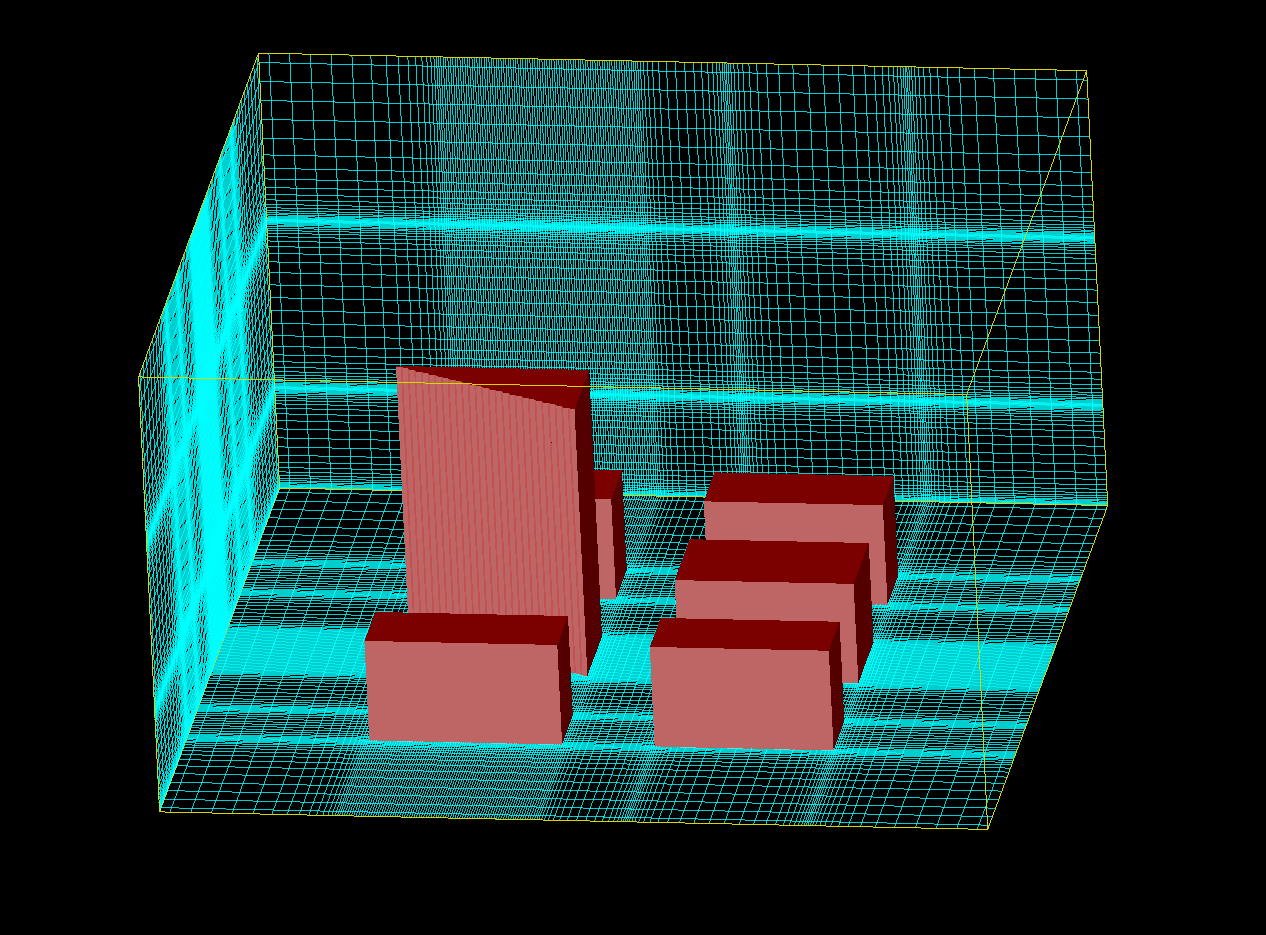
\includegraphics[width = \textwidth]{mesh.png}
\caption{The obstacles and mesh used in the analysis}
\label{fig:mesh}
\end{figure}
\subsection{Reynolds Number}
\subsection{Fluid properties}